\section{Sensors in Autonomous Vehicles}
With the help of sensors, autonomous vehicles ensure no human interaction is needed while driving. A wide range of sensors are used in autonomous vehicles to build reliable vision. The sensors help the self-driving vehicle to detect hurdles or blockages in the driving environment and to move without causing fatalities.
\\
Below are some primary sensors used in autonomous vehicles:

\subsection{Camera}
Cameras used in autonomous cars are specialized image sensors that detect the visible light spectrum reflected from objects. Cameras are the best sensor solution to give an accurate visual representation of an autonomous vehicle's surroundings. In autonomous vehicles, cameras are fixed on all four sides—front, rear, right, and left—to give a 360° view. These cameras use wide and narrow fields of view to perceive both short-range wide view and long-range arrow view. Super-wide lenses are used in autonomous vehicles for capturing a panoramic view that assists with parking. However, accurate camera visuals fail to give information regarding the distance of objects from autonomous vehicles.

\subsection{LiDAR}
LiDAR uses laser beams (light waves) to determine the distance between two objects. In autonomous vehicles, LiDAR is mounted on top of vehicles and is rotated at high speed while emitting laser beams. The laser beams reflect from the obstacles and travel back to the device. The time taken for this to happen is used to determine the distance, shape, and depth of the obstacles surrounding the autonomous vehicle.
\\
Even though LiDAR can catch the position, shape, size, and depth of an obstacle, they can get glitched by fake echoes showing far objects as near objects and vice versa. LiDAR fails to distinguish between multiple copies of laser signals and shows non-existent obstacles to autonomous vehicles. LiDAR does not function well in rain, snow, or fog. 

\subsection{RADAR}
The principle of operation for LiDAR and RADAR are the same, but instead of the light waves used in LIDAR, RADAR relies on radio waves. The time taken by the radio waves to return from the obstacles to the device is used for calculating the distance, angle, and velocity of the obstacle in the surroundings of the autonomous vehicle.
\\
RADAR in autonomous vehicles operates at the frequencies of 24, 74, 77, and 79 GHz, corresponding to short-range radars (SRR), medium-range radars (MRR), and long-range radars (LRR), respectively. They each have slightly different functions:
\begin{itemize}
    \item SRR technology enables blind-spot monitoring, lane-keeping assistance, and parking assistance in autonomous vehicles. 
    \item MRR sensors are used when obstacle detection is in the range of 100-150 meters with a beam angle varying between 30° to 160°. 
    \item The automatic distance control and brake assistance are supported by LRR radar sensors. 
\end{itemize}
RADAR technology in autonomous vehicles operates with millimeter waves and offers millimeter precision. The utilization of millimeter waves in autonomous vehicular RADAR ensures high resolution in obstacle detection and centimeter accuracy in position and movement determination. Compared to other sensor technologies in autonomous vehicles, RADAR works reliably under low visibility conditions such as cloudy weather, snow, rain, and fog. 

\subsection{Microphone}
A microphone is a transducer that converts sound into an electrical signal. Microphones are used to give hearing abilities to autonomous vehicles. In autonomous vehicles, microphones can be used to detect horns, emergency sirens, etc.
\\
Microphones in autonomous vehicles are also used to identify the condition of road, the vehicle is driving on. It is shown that different types of roads (like wet, sandy, snowy) have different spectrum hence plays an important role in the identification.

\section{Navigation Systems in Autonomous Vehicles}
Autonomous vehicles can use navigation systems to geolocate with numerical coordinates (e.g. latitude, longitude) representing their physical locations in space. They can also navigate by combining real-time GPS coordinates with other digital map data (e.g. via Google Maps).
\\
Geolocation data often varies around a five-meter radius. To compensate for imprecise GPS data, self-driving cars can use unique data-processing techniques like particle filtering to improve location accuracy. Furthermore, these systems can also be used to make efficient judgement for vehicle to take turn.
\\
Some geolocation services used nowadays includes  Indian Regional Navigation Satellite System (\textit{IRNSS} or \textit{NavIC}), United States' Global Positioning System (\textit{GPS}), Russia's Global Navigation Satellite System (\textit{GLONASS}), China's \textit{BeiDou} Navigation Satellite System and the European Union's \textit{Galileo}.

\section{Vehicle Control with Deep Learning}
Artificial Intelligence is the major backbone of the autonomous vehicles which enables vehicle to recognize and react to their environment in real time, allowing them to safely navigate. This is called \textbf{Perception}, the ability, while driving, to process and identify road data — from street signs to pedestrians to surrounding traffic.
\\
In the earlier stages, Machine Learning was used to enable vehicles to perceive their environment. But as the technology increases, Deep Learning or use of Neural Networks turns out to be the better approach for the classification.

\subsection{Machine Learning vs Deep Learning}
\subsubsection{Machine Learning}
Machine Learning is an application of artificial intelligence that includes algorithms that parse data, learn from that data, and then apply what they've learned to make informed decisions.
\\
In machine learning, human intervention is needed to extract the features based on input to make the accurate predictions. Furthermore, if an AI algorithm returns an inaccurate prediction, then an engineer has to step in and make adjustments.

\subsubsection{Deep Learning}
Deep Learning is subfield of machine learning that structures algorithms in layers to create an “artificial neural network” that can learn and make intelligent decisions on its own.
\\
A deep learning model is designed to continually analyze data with a logical structure similar to how a human would draw conclusions. To complete this analysis, deep learning applications use a layered structure of algorithms called an \textbf{Artificial Neural Network}. The design of an artificial neural network is inspired by the biological network of neurons in the human brain, leading to a learning system that's far more capable than that of standard machine learning models
\\
\\
Figure 2.1 shows the distinction between algorithms based on Machine Learning and Deep Learning.

\begin{figure}[h]
    \centering
    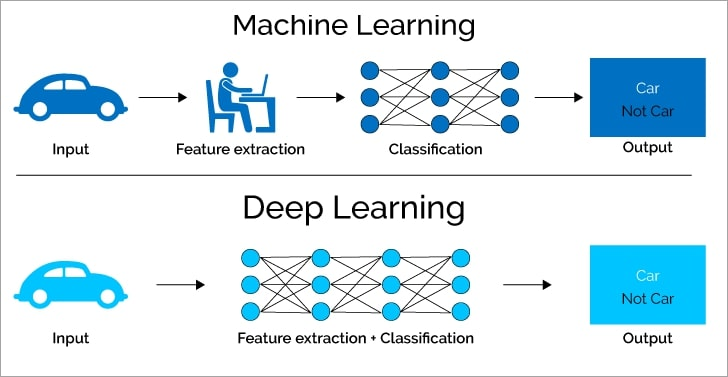
\includegraphics[width = 5in]{Ch02/ml_vs_dl.png}
    \caption{Difference Between Machine Learning and Deep Learning}
    \label{figure:9}
\end{figure}
\FloatBarrier

\subsubsection{Machine Learning or Deep Learning for Autonomous Vehicles}
In case of autonomous vehicles, rather than requiring a manually written set of rules for the car to follow, such as “stop if you see red,” Neural Networks enable vehicles to learn how to navigate the world on their own using sensor data. This makes Deep Learning algorithms optimal as the decision maker for the autonomous vehicle. 

\subsection{Deep Learning Algorithms}
In the field of computer vision, over the period of time, several algorithms or neural networks are designed like Convulational Neural Networks, Generative Adversarial Networks, Transformers. With the advancement in technologies, advancement in accuracy of each neural network is done with transformers currently as the algorithms making best predictions.

\subsubsection{Transformer Networks}
Transformer networks have been proven to achieve better accuracy in a variety of autonomous vehicle perception tasks when compared to convolutional neural networks running on embedded systems.
\\
First transformer network (say, native transformer)\cite{2017arXiv170603762V} has 3 major components:
\begin{enumerate}
    \item Positional Embeddings
    \item Transformer Encoder
    \item Transformer Decoder
\end{enumerate}
This network was formed to performe tasks in the field of Natural Language Processing. After further research, a new transformer named \textbf{Vision Transformer}\cite{dosovitskiy2021image} was built to perform tasks related to Computer Vision.
\\
In Vision Transformer, the Encoder has remained same but the algorithms for Positional Embeddings and Decoder were changed.
For autonomous vehicles, since computer vision plays an important role, the model designing is inspired using Vision Transformer

\subsubsection{Positional Embedder in Vision Transformer}
As shown in the figure 2.2, in positional embedding layer, the image is first split into fixed-size patches, then each patch linearly embedded,
add finally position embeddings are done, and the resulting sequence of vectors are fed to a standard Transformer encoder.
\begin{figure}[h]
    \centering
    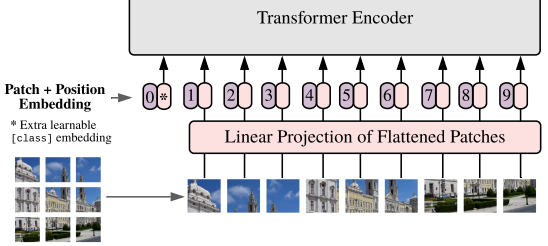
\includegraphics[width = 4in]{Ch02/positional_embedding.png}
    \caption{Positional Embedding Layer used in Vision Transformer}
    \label{figure:10}
\end{figure}
\FloatBarrier

\subsubsection{Encoder in Vision Transformer}
The encoder is composed of a stack of N identical layers. Each layer has two sub-layers. The first is a multi-head self-attention mechanism, and the second is a simple, position-wise fully connected feed-forward network. A residual connection is employed around each of the two sub-layers, followed by Layer Normalization\cite{ba2016layer}.
\\
Figure 2.3 shows the encoder used in Vision Transformer.
\begin{figure}[h]
    \centering
    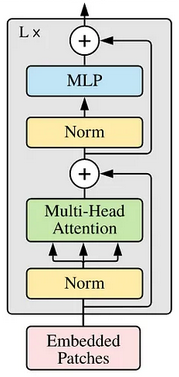
\includegraphics[width = 2in]{Ch02/transformer_encoder.png}
    \caption{Encoder used in Vision Transformer}
    \label{figure:11}
\end{figure}
\FloatBarrier

\subsubsection{Multi-Head Attention in Transformers}
Multi-head Attention is a module for attention mechanisms which runs through an attention mechanism several times in parallel. The independent attention outputs are then concatenated and linearly transformed into the expected dimension. Intuitively, multiple attention heads allows for attending to parts of the sequence differently (e.g. longer-term dependencies versus shorter-term dependencies).
\[ MultiHead(Q, K, V) = [head_1,...,head_h]W_o \]
\[ where \; head_i = Attention(QW_i^Q, KW_i^K, VW_i^V) \]
In the above eqaution, W is the learning prameter and Attention is a mathematical function from Scaled Dot-Product Attention which is a single attention layer or a head in multi-head attention layer.
\\
Scaled dot-product attention is an attention mechanism where the dot products are scaled down by \(\sqrt{d_k}\). Formally we have a query \(Q\), a key \(K\) and a value \(V\) and calculate the attention as:
\[ Attention(Q,K,V) = softmax\left(\frac{QK^T}{\sqrt{d_k}}\right)V \]
With the help of Multi-Head Attention in Encoder, each position in the encoder can attend to all positions in the previous layer of the encoder. This played a mojor role in making Transformers more efficient and thus formed a backbone for the Transformers.

\subsubsection{Multi-Layer Perceptron in Transformers}
Multi layer perceptron (MLP) is a supplement of feed forward neural network. It consists of three types of layers—the input layer, output layer and hidden layer. The input layer receives the input signal to be processed. The required task such as prediction and classification is performed by the output layer. An arbitrary number of hidden layers that are placed in between the input and output layer are the true computational engine of the MLP. Similar to a feed forward network in a MLP the data flows in the forward direction from input to output layer.
\\
The Multi-layer perceptron used in vision transformer contains GELU non-linearity\cite{hendrycks2020gaussian}. Since the encoder block repeats, we have to be careful about the number of units in the hidden layer because the output dimension has to be compatible with the input for the next MultiHeadAttention layer.

\subsubsection{Decoder in Vision Transformer}
Decoder as per the paper is a normal classifier in which the tensor passed from the encoder are passed first through a Multi-Layer Perceptron and then with the help of softmax activation, classification was done.
\\
Figure 2.4 describes the classifier used as decoder in the transformer.
\begin{figure}[h]
    \centering
    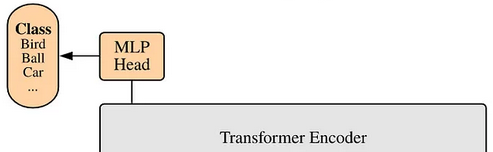
\includegraphics[width = 4in]{Ch02/transformer_decoder.png}
    \caption{Decoder used in Vision Transformer}
    \label{figure:12}
\end{figure}
\FloatBarrier